\documentclass[8pt]{beamer}
\usepackage[]{graphicx}
\usepackage[]{color}


\usetheme{metropolis}           % Use metropolis theme
\usepackage{amsmath}
\usepackage{mathrsfs}
\usepackage{tabularx}

\usepackage[style=authoryear]{biblatex}
\addbibresource{references.bib}
\usepackage{cleveref}
\renewcommand*{\bibfont}{\footnotesize}


\title{Budget Deep Dive}
\author{Ryan Giordano}
\date{Sep 23rd, 2022}
\institute{Children's Community Center}

\begin{document}




%%%%%%%%%%%%%%%%%%%%%%%%%%%%%%%%%%%%%%%%%%%%%%%%%%%%%%%%%%%%%%%%%%%%%%%
%%%%%%%%%%%%%%%%%%%%%%%%%%%%%%%%%%%%%%%%%%%%%%%%%%%%%%%%%%%%%%%%%%%%%%%
%%%%%%%%%%%%%%%%%%%%%%%%%%%%%%%%%%%%%%%%%%%%%%%%%%%%%%%%%%%%%%%%%%%%%%%

\begin{frame}{Outline}

Here are some questions you might have:
%
\begin{itemize}
%
\item Ryan, do we have money for this thing I want to do?
\item How is that that we have so much money in the bank, especially after COVID?
\item If we have so much money in the bank, why didn't we give the teachers
    a raise?
\item How does the budget get set anyway, and how good are we at meeting it?
\item How will equity tuition change all of this?
%
\end{itemize}
%
I will try to sketch answers to these questions today.
%
\end{frame}

%%%%%%%%%%%%%%%%%%%%%%%%%%%%%%%%%%%%%%%%%%%%%%%%%%%%%%%%%%%%%%%%%%%%%%%
%%%%%%%%%%%%%%%%%%%%%%%%%%%%%%%%%%%%%%%%%%%%%%%%%%%%%%%%%%%%%%%%%%%%%%%
%%%%%%%%%%%%%%%%%%%%%%%%%%%%%%%%%%%%%%%%%%%%%%%%%%%%%%%%%%%%%%%%%%%%%%%

\begin{frame}{Who are the budgeteers?}
%
\begin{itemize}
%
\item Vidrik Frankfather, our staff accountant.
\begin{itemize}
    \item A past CCC parent and board treasurer
    \item Has actual accounting expertise
    \item Discovered errors in the work done by our contracted accounting firm,
        suggested that he could do it better as a part-time staff member
    \item A great repository of detailed information and historical context
\end{itemize}
%
%
\item Edna Tow, our school manager.
\begin{itemize}
    \item Also a past CCC parent
    \item Collects tuition, pays salaries, processes reimbursements
    \item Manages bank accounts and investments
    \item A great repository of detailed information and historical context
\end{itemize}
%
%
\item Board treasurer (whomever they may be)
\begin{itemize}
    \item May not have actual accounting experience
    \item May not know a lot of historical context
    \item May not have even been present when the last budget was passed
    \item Facilitates communication between parents, the board, the teachers,
        and the staff who actually know what they are doing
\end{itemize}
%
\end{itemize}
%
\end{frame}



%%%%%%%%%%%%%%%%%%%%%%%%%%%%%%%%%%%%%%%%%%%%%%%%%%%%%%%%%%%%%%%%%%%%%%%
%%%%%%%%%%%%%%%%%%%%%%%%%%%%%%%%%%%%%%%%%%%%%%%%%%%%%%%%%%%%%%%%%%%%%%%
%%%%%%%%%%%%%%%%%%%%%%%%%%%%%%%%%%%%%%%%%%%%%%%%%%%%%%%%%%%%%%%%%%%%%%%

\begin{frame}{What goes into our budget?}
%
Our income is almost all tuition, and our expenses are almost all salaries.

For example, in the 2018-2019 school year:
%
\begin{itemize}
%
\item Total income was $\sim$ \$594k
\begin{itemize}
    \item 91\% came from tuition ($\sim 2/3$ of this came from AM tuition)
    % \item 63\% came from AM tuition
    % \item 29\% came from ``contract care'' (PM1, PM2, etc.)
    % \item 8\% came from fees and donations
\end{itemize}
%
\item Total expenditures were $\sim$ \$568k
\begin{itemize}
    \item 87\% went to personnel
\end{itemize}
%
\end{itemize}
%

It is difficult to raise teachers' salaries without
raising tuition a comparable amount.

This led to our current policy on teacher raises and bonuses (PPM page 28):

% {\em
% %
% ``Historically, CCC employed a traditional step scale merit system to raise
% teacher salaries. ... [H]owever, this system caused a serious financial strain on
% the school. ... To remain competitive, in 2008 the Board of Directors froze the
% salaries of several long standing employees and ceased the use of the step scale
% system to calculate raises. ... Since that time, teachers have had no mechanism
% to increase their salary, short of a Board of Directors-approved cost of living
% adjustment.  In years of prosperity, teachers should be given a generous share
% [of any budget surplus] to make up for years when such generosity was not
% possible.''
% %
% }
%
\begin{itemize}
%
\item Teachers get a COLA increase, but do not get raises.
\item  When we have a surplus we are supposed to:
\begin{itemize}
\item \textcolor{red}{Give teachers generous bonuses.}
\item \textcolor{red}{Fund the employee endowment fund (EEF).}
\end{itemize}
%
\end{itemize}
%

So how often / how much do we have surpluses?

% The first two years of COVID19 were different, as we will discuss later.
%
\end{frame}


%%%%%%%%%%%%%%%%%%%%%%%%%%%%%%%%%%%%%%%%%%%%%%%%%%%%%%%%%%%%%%%%%%%%%%%
%%%%%%%%%%%%%%%%%%%%%%%%%%%%%%%%%%%%%%%%%%%%%%%%%%%%%%%%%%%%%%%%%%%%%%%
%%%%%%%%%%%%%%%%%%%%%%%%%%%%%%%%%%%%%%%%%%%%%%%%%%%%%%%%%%%%%%%%%%%%%%%

\begin{frame}{Budget over time}
\begin{figure}
\begin{center}
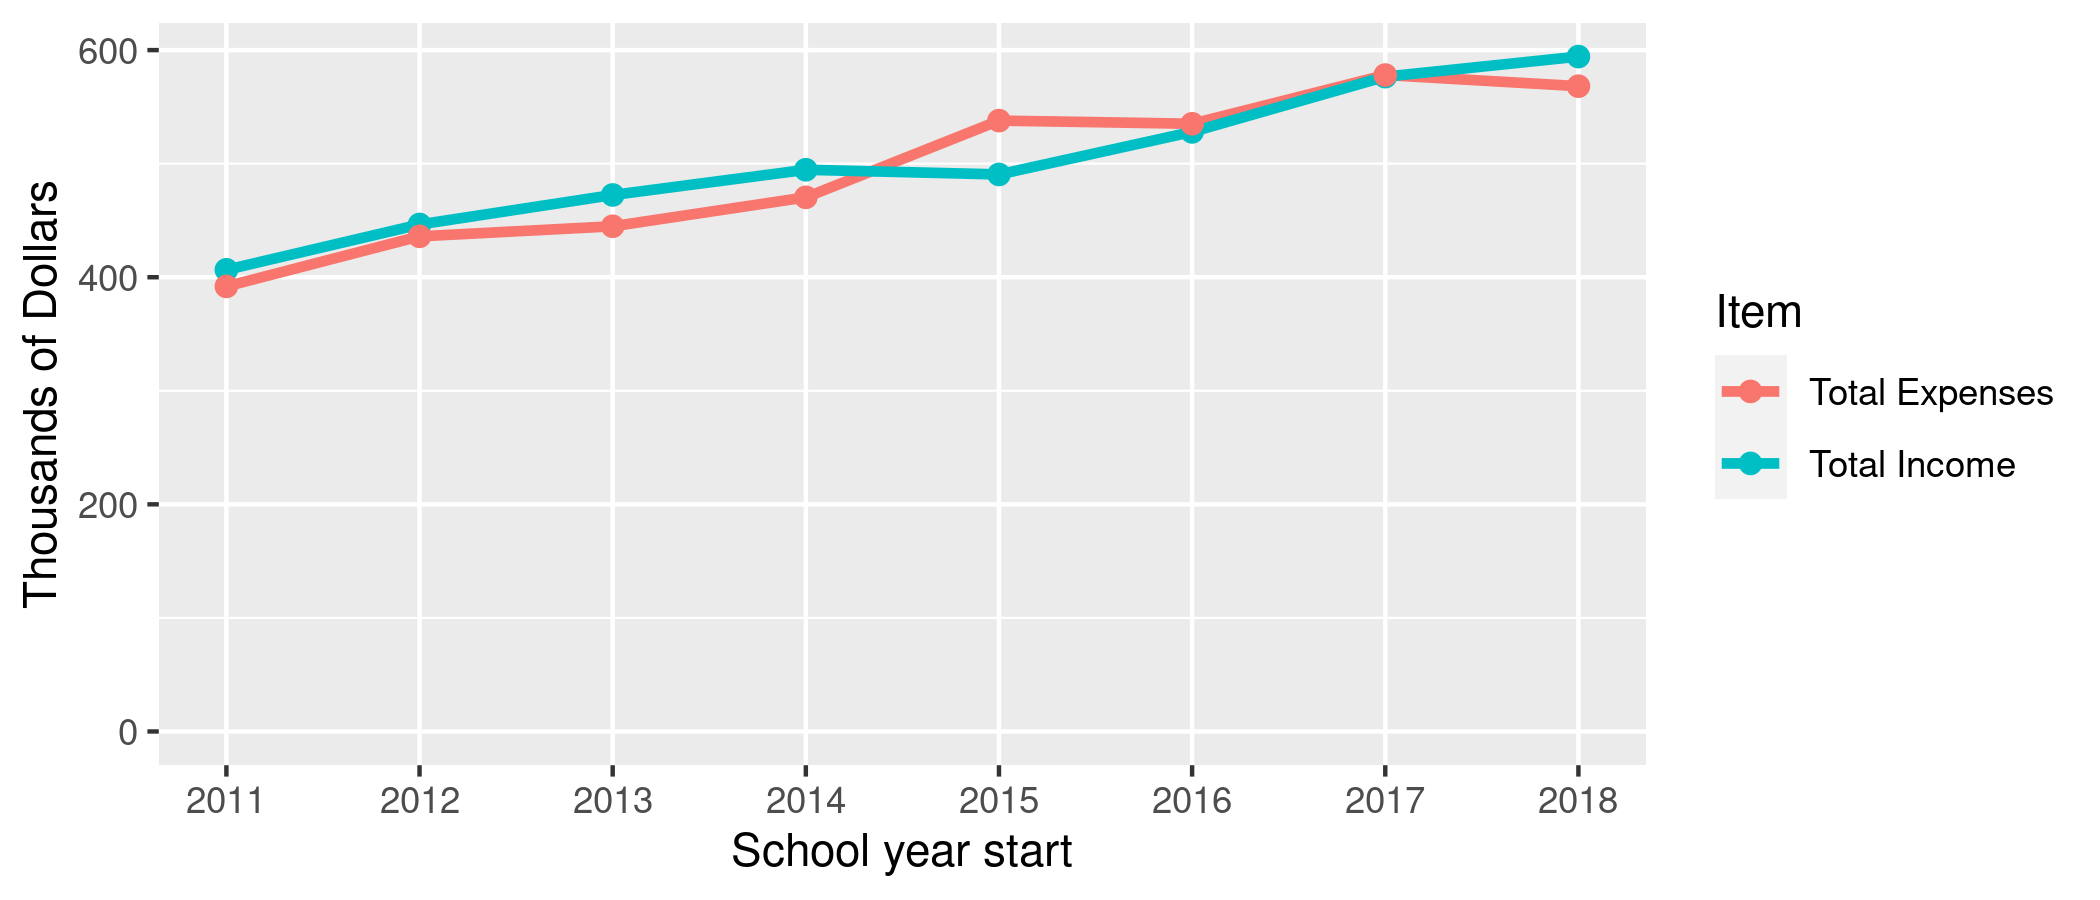
\includegraphics[width=3in]{budget_history.png}
\end{center}
\end{figure}

Between the 2011-2012 and 2018-2019 school years (inclusive):
%
\begin{itemize}
%
\item Actual income ran from $\sim$ \$400k - \$600k
\item The largest defecit was \$47k (10\%), and the largest surplus \$28k (4\%)
% \item These were 10\% and 4\% of revenue, respectively
\item Over all these years, the net surplus was \$47k ($\sim$\$6k or 1.2\% / year)
\item Typical variability was from a 0.5\% loss to 4.5\% surplus (IQR)
\item We met the budget 63\% of the time (5/8)
%
\end{itemize}
%
\textcolor{red}{Because we run a tight budget, we have
under-invested in B\&G and teacher bonuses.}

\textbf{Story of the \$47k loss:}
In 2015, a B\&G project went over budget, causing the board to mandate
increasing the required cash reserve from 10\% to 20\%.
(PPM Article IX)
Vidrik (then treasurer) created a 10-year plan to save the difference.

\end{frame}


%%%%%%%%%%%%%%%%%%%%%%%%%%%%%%%%%%%%%%%%%%%%%%%%%%%%%%%%%%%%%%%%%%%%%%%
%%%%%%%%%%%%%%%%%%%%%%%%%%%%%%%%%%%%%%%%%%%%%%%%%%%%%%%%%%%%%%%%%%%%%%%
%%%%%%%%%%%%%%%%%%%%%%%%%%%%%%%%%%%%%%%%%%%%%%%%%%%%%%%%%%%%%%%%%%%%%%%


\begin{frame}{Budget over time: COVID years}
\begin{figure}
\begin{center}
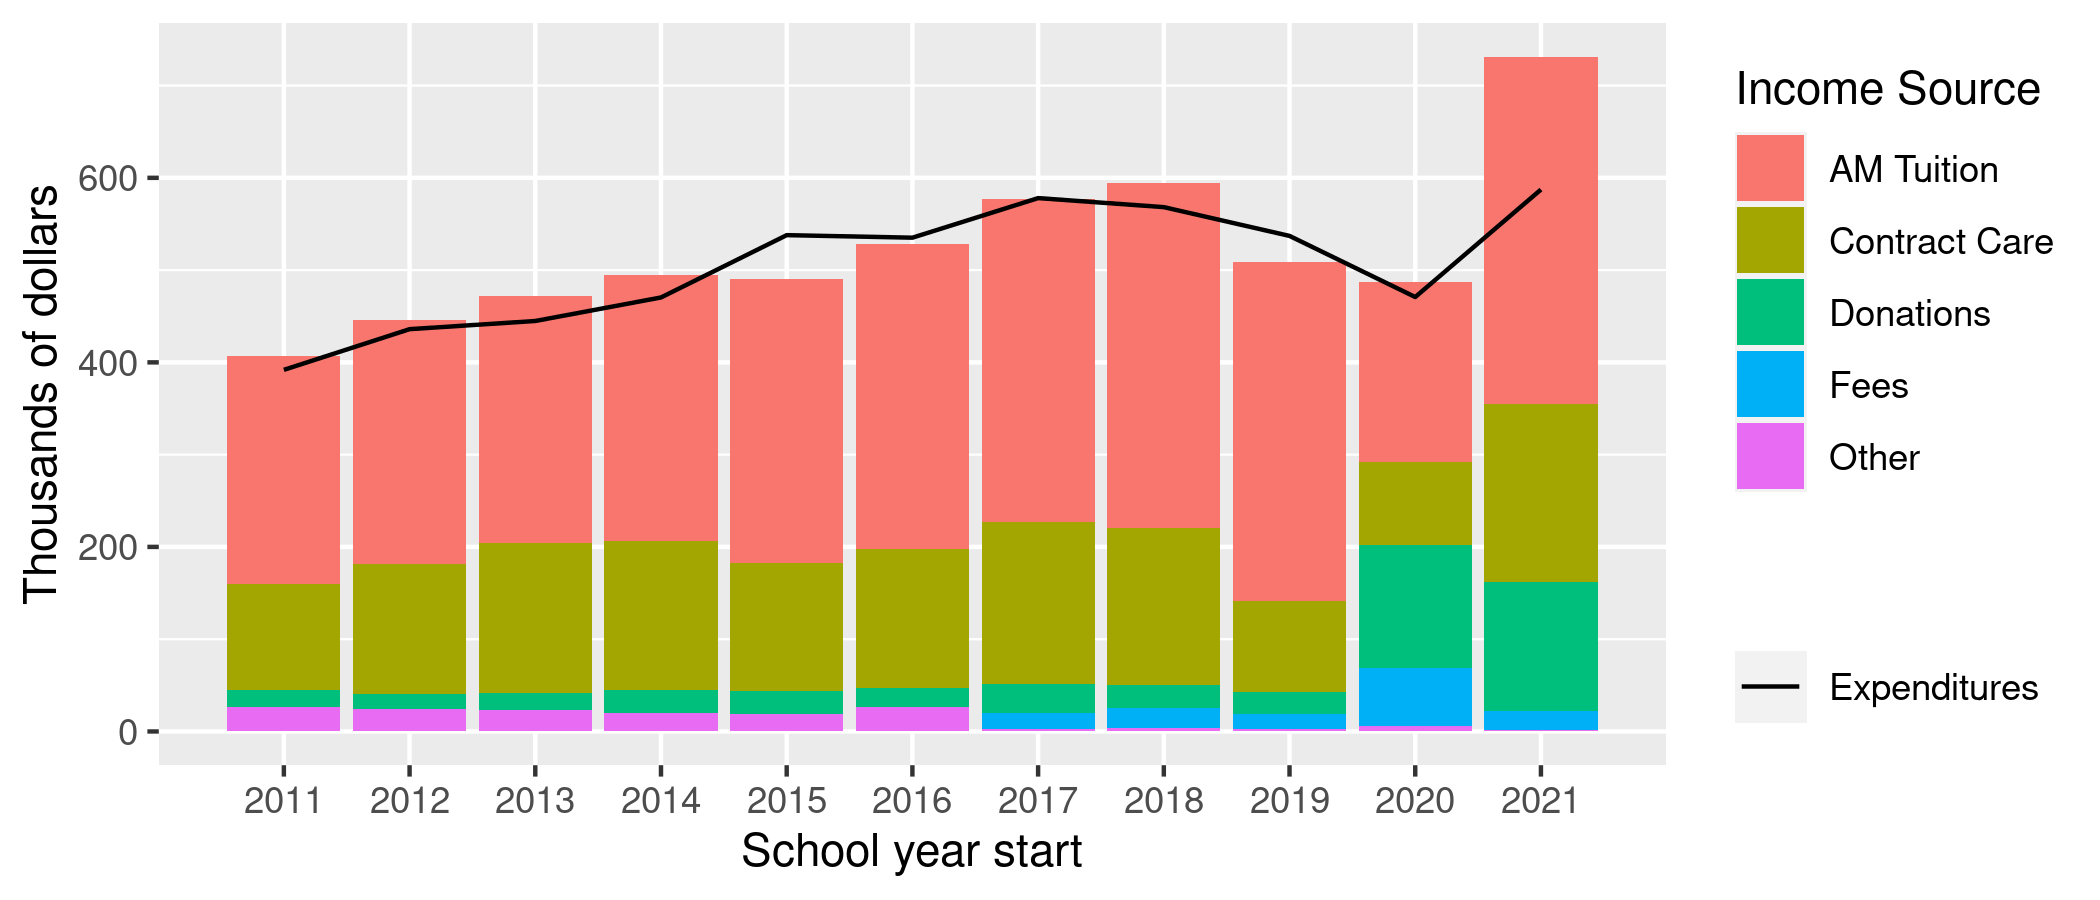
\includegraphics[width=3in]{budget_history_w_income_source.png}
\end{center}
\end{figure}

When COVID hit (midway through the 2019-2020 school year):
%
\begin{itemize}
%
\item We charged normal tuition for 2019-2020
\item Tuition dropped off {\em steeply} 2020-2021 (partial shutdown)
\item The shortfall was made up (and then some) from {\em one-time donations}:
\begin{itemize}
    \item Past families
    \item Corporate donations
    \item Government assistance (e.g. forgiven paychek protection loans)
\end{itemize}
\item As a result, we emerged from COVID19 with a large, one-time surplus.
%
\end{itemize}
%
The surplus first went to the 20\% reserve.
\textbf{Currently, about \$330k remains}.

Why didn't the teachers get a big bonus in 2021?  After subtracting one-time
donations, the surplus was only $\sim$\$5k, less than 1\% of budget.

\end{frame}


%%%%%%%%%%%%%%%%%%%%%%%%%%%%%%%%%%%%%%%%%%%%%%%%%%%%%%%%%%%%%%%%%%%%%%%
%%%%%%%%%%%%%%%%%%%%%%%%%%%%%%%%%%%%%%%%%%%%%%%%%%%%%%%%%%%%%%%%%%%%%%%
%%%%%%%%%%%%%%%%%%%%%%%%%%%%%%%%%%%%%%%%%%%%%%%%%%%%%%%%%%%%%%%%%%%%%%%


\begin{frame}{How is the budget made?}

% PPP (Article IV, and Membership Meetings):
%
% {\em
% ``The Treasurer shall submit a proposed budget for approval at the April Budget
% Adoption Meeting. To be adopted, the budget must be approved by a majority of
% those present. ... A Budget Adoption Meeting shall be held in April. The
% presence of one-third (1/3) of the membership of the corporation then
% outstanding at any meeting shall constitute a quorum.''
% }

In practice, I understand that, in the April board meeting:
%
\begin{enumerate}
%
\item Vidrik and the treasurer present several (2 or 3) potential scenarios.
\begin{itemize}
    \item Scenarios vary capital expenditures, savings, \&c
    \item Teachers get a cost-of-living (COLA) increase every year
    \item The scenarios increase or decrease tuition to match expenses
\end{itemize}
\item The board approves the scenarios, which are then sent for an all-school
vote.
%
\end{enumerate}
%

In the past, tuition was set directly, typically as a small increase over
the previous year.

After equity tuition, we will not set tuition directly.  Instead we will:
%
\begin{enumerate}
%
\item Make our budget scenarios without looking at the income of incoming
families,
\item After seeing the income distribution, set the \% of income that will cover
expenditures for each scenario,
\item If the required \% of income would be too large (e.g. $> 5\%$)
make up the difference from an {\em equity tuition reserve}.
%
\end{enumerate}
%
Some consequences of equity tuition:
%
\begin{itemize}
%
\item Equity tuition may make it more palatable to regularly run a surplus.
\item Equity tuition will increase income volatility
    (I estimate at least $\pm 7\%$ of budget).
\item \textcolor{red}{We will need to save to fill up the reserve.}
%
\end{itemize}
%
\end{frame}


%%%%%%%%%%%%%%%%%%%%%%%%%%%%%%%%%%%%%%%%%%%%%%%%%%%%%%%%%%%%%%%%%%%%%%%
%%%%%%%%%%%%%%%%%%%%%%%%%%%%%%%%%%%%%%%%%%%%%%%%%%%%%%%%%%%%%%%%%%%%%%%
%%%%%%%%%%%%%%%%%%%%%%%%%%%%%%%%%%%%%%%%%%%%%%%%%%%%%%%%%%%%%%%%%%%%%%%

\begin{frame}{How to use the COVID19 surplus?}

\textbf{Currently, about \$330k of the COVID19 windfall remains}.

\textbf{Big TODO for all of us: Decide what (if
anything) to do with this surplus.}

Three immediate suggestions (which were \textcolor{red}{colored red above}):
%
\begin{enumerate}
%
\item Investing in buildings and grounds
\item Giving the teachers a bonus / funding the employee endowment fund
\item Jump-starting the equity tuition fund
%
\end{enumerate}
%
\textbf{Now is a good idea to start talking about your ideas!}


\end{frame}

\end{document}
